\section{Introdução ao Controle Digital}

\begin{frame}{Introdução}
\begin{block}{}
\begin{itemize}
	\item Controle de sistemas físicos com uso de um computador digital.
	\item Estudado até agora: tempo contínuo para implementação analógica (hidráulico, pneumático, eletrônico analógico).
	\item Avanço do uso da tecnologia de \textbf{microprocessadores}.
\end{itemize}

\textbf{Objetivo:} Projetar controladores digitais para obter uma boa resposta dinâmica e minimizar o erro no controle com sinais digitais.

\end{block}
\end{frame}

\begin{frame}{Sinais}

\begin{minipage}{0.48\linewidth}
	\centering
	
	\scalebox{0.5}{

\tikzset{every picture/.style={line width=0.75pt}} %set default line width to 0.75pt        

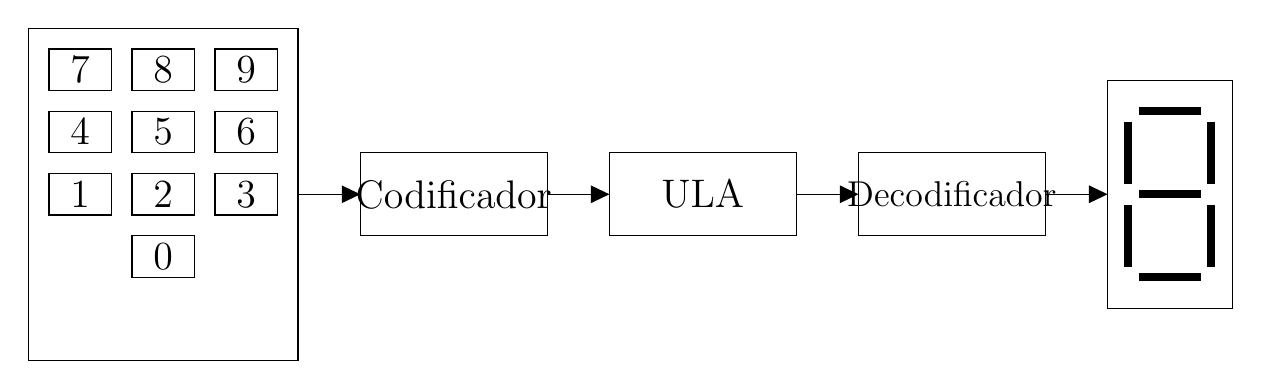
\begin{tikzpicture}[x=0.75pt,y=0.75pt,yscale=-1,xscale=1]
%uncomment if require: \path (0,300); %set diagram left start at 0, and has height of 300

%Shape: Rectangle [id:dp8798188650405219] 
\draw   (30,50) -- (160,50) -- (160,210) -- (30,210) -- cycle ;
%Shape: Rectangle [id:dp593444354888008] 
\draw   (40,60) -- (70,60) -- (70,80) -- (40,80) -- cycle ;
%Shape: Rectangle [id:dp4412846627526852] 
\draw   (80,60) -- (110,60) -- (110,80) -- (80,80) -- cycle ;
%Shape: Rectangle [id:dp2343273962035186] 
\draw   (120,60) -- (150,60) -- (150,80) -- (120,80) -- cycle ;
%Shape: Rectangle [id:dp05777918912875246] 
\draw   (40,90) -- (70,90) -- (70,110) -- (40,110) -- cycle ;
%Shape: Rectangle [id:dp9955010424516375] 
\draw   (80,90) -- (110,90) -- (110,110) -- (80,110) -- cycle ;
%Shape: Rectangle [id:dp24021539717259266] 
\draw   (120,90) -- (150,90) -- (150,110) -- (120,110) -- cycle ;
%Shape: Rectangle [id:dp36169684584711925] 
\draw   (40,120) -- (70,120) -- (70,140) -- (40,140) -- cycle ;
%Shape: Rectangle [id:dp7232437677097003] 
\draw   (80,120) -- (110,120) -- (110,140) -- (80,140) -- cycle ;
%Shape: Rectangle [id:dp6884539525496838] 
\draw   (120,120) -- (150,120) -- (150,140) -- (120,140) -- cycle ;
%Shape: Rectangle [id:dp9961423077173726] 
\draw   (80,150) -- (110,150) -- (110,170) -- (80,170) -- cycle ;
%Shape: Rectangle [id:dp6643057105712631] 
\draw   (190,110) -- (280,110) -- (280,150) -- (190,150) -- cycle ;
%Shape: Rectangle [id:dp7094011053258715] 
\draw   (550,75) -- (610,75) -- (610,185) -- (550,185) -- cycle ;
%Shape: Rectangle [id:dp2693438921699036] 
\draw   (310,110) -- (400,110) -- (400,150) -- (310,150) -- cycle ;
%Shape: Rectangle [id:dp3654960401722005] 
\draw   (430,110) -- (520,110) -- (520,150) -- (430,150) -- cycle ;
%Straight Lines [id:da6667328032348829] 
\draw    (160,130) -- (188,130) ;
\draw [shift={(190,130)}, rotate = 180] [fill={rgb, 255:red, 0; green, 0; blue, 0 }  ][line width=0.75]  [draw opacity=0] (8.93,-4.29) -- (0,0) -- (8.93,4.29) -- cycle    ;

%Straight Lines [id:da5165651690517046] 
\draw    (280,130) -- (308,130) ;
\draw [shift={(310,130)}, rotate = 180] [fill={rgb, 255:red, 0; green, 0; blue, 0 }  ][line width=0.75]  [draw opacity=0] (8.93,-4.29) -- (0,0) -- (8.93,4.29) -- cycle    ;

%Straight Lines [id:da17751850693095572] 
\draw    (400,130) -- (428,130) ;
\draw [shift={(430,130)}, rotate = 180] [fill={rgb, 255:red, 0; green, 0; blue, 0 }  ][line width=0.75]  [draw opacity=0] (8.93,-4.29) -- (0,0) -- (8.93,4.29) -- cycle    ;

%Straight Lines [id:da4998570413390182] 
\draw [color={rgb, 255:red, 0; green, 0; blue, 0 }  ,draw opacity=1 ][line width=3]    (560,95) -- (560,125) ;


%Straight Lines [id:da05287212083080073] 
\draw [color={rgb, 255:red, 0; green, 0; blue, 0 }  ,draw opacity=1 ][line width=3]    (600,95) -- (600,125) ;


%Straight Lines [id:da9146969001147236] 
\draw [color={rgb, 255:red, 0; green, 0; blue, 0 }  ,draw opacity=1 ][line width=3]    (560,135) -- (560,165) ;


%Straight Lines [id:da37610179690179124] 
\draw [color={rgb, 255:red, 0; green, 0; blue, 0 }  ,draw opacity=1 ][line width=3]    (600,135) -- (600,165) ;


%Straight Lines [id:da2798262228013664] 
\draw [color={rgb, 255:red, 0; green, 0; blue, 0 }  ,draw opacity=1 ][line width=3]    (595,130) -- (565,130) ;


%Straight Lines [id:da15184615547446478] 
\draw [color={rgb, 255:red, 0; green, 0; blue, 0 }  ,draw opacity=1 ][line width=3]    (595,90) -- (565,90) ;


%Straight Lines [id:da20609816632014244] 
\draw [color={rgb, 255:red, 0; green, 0; blue, 0 }  ,draw opacity=1 ][line width=3]    (595,170) -- (565,170) ;


%Straight Lines [id:da16937059284664002] 
\draw    (520,130) -- (548,130) ;
\draw [shift={(550,130)}, rotate = 180] [fill={rgb, 255:red, 0; green, 0; blue, 0 }  ][line width=0.75]  [draw opacity=0] (8.93,-4.29) -- (0,0) -- (8.93,4.29) -- cycle    ;


% Text Node
\draw (135,70) node   {\Large $9$};
% Text Node
\draw (95,70) node   {\Large $8$};
% Text Node
\draw (55,70) node   {\Large $7$};
% Text Node
\draw (135,100) node   {\Large $6$};
% Text Node
\draw (135,130) node   {\Large $3$};
% Text Node
\draw (95,160) node   {\Large $0$};
% Text Node
\draw (95,130) node   {\Large $2$};
% Text Node
\draw (95,100) node   {\Large $5$};
% Text Node
\draw (55,100) node   {\Large $4$};
% Text Node
\draw (55,130) node   {\Large $1$};
% Text Node
\draw (235,130) node  [align=left] {\Large Codificador};
% Text Node
\draw (355,130) node  [align=left] {\Large ULA};
% Text Node
\draw (475,130) node [scale=0.9] [align=left] {\Large Decodificador};


\end{tikzpicture}
}
	
	Sinal em tempo contínuo e analógico
\end{minipage}\tikzmark{ar1}
\hfill
\begin{minipage}{0.48\linewidth}
	\centering
	
	\scalebox{0.5}{\deftkzbds
	
\begin{tikzpicture}[auto, node distance=2cm,>=Latex]
	
	\node [input, name=input] {};
	
	\node [coordinate, right=of input] (junction) {};
	\draw (input) -- node[near start] {$E(z)$} (junction);
	
	\node [block, right=of junction] (ei) {$ C_i(z) $};
	\node [block, above=of ei] (kp) {$ C_p(z) $};
	\node [block, below=of ei] (cd) {$ C_d(z) $};
	
	\draw [->] (junction) -- (ei);
	\draw [->] (junction) |- (kp);
	\draw [->] (junction) |- (cd);
	
	\node [sum, right=2cm of ei] (sum) {$ \phantom{\sum} $};
	\draw (sum) ++(-8pt,-8pt) -- ++(16pt,16pt) ++(-16pt,0pt) -- +(16pt,-16pt);
	
	\draw [<-] (sum) -- node[very near start, above] {$ + $} (ei);
	\draw [<-] (sum) |- node[very near start, right] {$ + $} (kp);
	\draw [<-] (sum) |- node[very near start, left] {$ + $} (cd);
	
	\node [output, right=of sum] (output) {};
	\draw [->] (sum) -- node[near end] {$ U(z) $} (output);
\end{tikzpicture}}
	
	Sinal em tempo discreto e analógico
\end{minipage}

\begin{tikzpicture}[overlay, remember picture]
	\draw[-Implies, double distance=2pt] ($(ar1)+(-0.3,0)$) -- node[below] {\small Amostragem} +(0.8,0);
\end{tikzpicture}
	
\end{frame}


\begin{frame}{Sinais}
\begin{minipage}{0.48\linewidth}
	\centering
	
	\scalebox{0.5}{\deftkzbds
	
\begin{tikzpicture}[auto, node distance=2cm,>=Latex]
	
	\node [input, name=input] {};
	
	\node [coordinate, right=of input] (junction) {};
	\draw (input) -- node[near start] {$E(z)$} (junction);
	
	\node [block, right=of junction] (ei) {$ C_i(z) $};
	\node [block, above=of ei] (kp) {$ C_p(z) $};
	\node [block, below=of ei] (cd) {$ C_d(z) $};
	
	\draw [->] (junction) -- (ei);
	\draw [->] (junction) |- (kp);
	\draw [->] (junction) |- (cd);
	
	\node [sum, right=2cm of ei] (sum) {$ \phantom{\sum} $};
	\draw (sum) ++(-8pt,-8pt) -- ++(16pt,16pt) ++(-16pt,0pt) -- +(16pt,-16pt);
	
	\draw [<-] (sum) -- node[very near start, above] {$ + $} (ei);
	\draw [<-] (sum) |- node[very near start, right] {$ + $} (kp);
	\draw [<-] (sum) |- node[very near start, left] {$ + $} (cd);
	
	\node [output, right=of sum] (output) {};
	\draw [->] (sum) -- node[near end] {$ U(z) $} (output);
\end{tikzpicture}}
	
	Sinal em tempo discreto e analógico
\end{minipage}\tikzmark{ar1}
\hfill
\begin{minipage}{0.48\linewidth}
	\centering
	
	\scalebox{0.51}{%\begin{tikzpicture}[scale=1.5,>=latex, every node/.style={inner sep=2pt}]
%	
%	%\draw[pattern=north west lines, draw=mWhite] (0cm,0cm) circle(1cm);
%
%	\draw[dashed] (0cm,0cm) circle(1cm);
%	
%    % draw the coordinates
%    \draw[->, fill=white] (-1.5cm,0cm) -- (1.5cm,0cm) node[right=2pt] {$\Re(z)$};
%    \draw[->, fill=white] (0cm,-1.5cm) -- (0cm,1.5cm) node[above=2pt] {$\Im(z)$};
%    
%    \draw[->] (0,0) -- (45:1) node[right=2pt] {$ r=1 $};
%    
%    \draw[] (-1.4,0) ++(-2pt,-2pt) -- ++(4pt,4pt) ++(-4pt,0pt) -- ++(4pt,-4pt) +(-2pt,2pt) node[below=2pt, xshift=-3pt] {$ -1,4 $};
%    
%    \draw[fill=white] (-0.25,0) circle (1pt) node[below=2pt, xshift=-3pt] {$ -0,25 $};
%    
%    \draw[fill=white] (0,0) circle (1pt) node[below right=2pt] {$ 0 $};
%    
%    \draw[] (0.6,0) ++(-2pt,-2pt) -- ++(4pt,4pt) ++(-4pt,0pt) -- ++(4pt,-4pt) +(-2pt,2pt) node[below=2pt] {$ 0,6 $};
%\end{tikzpicture}


\begin{tikzpicture}[scale=1.5,>=latex, every node/.style={inner sep=2pt}]

\draw[pattern=south east lines, draw=mWhite] (0cm,0cm) circle(1.4cm);

\draw[dashed] (0cm,0cm) circle(1.4cm);

\draw[dashed, fill=white] (0cm,0cm) circle(0.6cm);

% draw the coordinates
\draw[->, fill=white] (-2cm,0cm) -- (2cm,0cm) node[right=2pt,fill=white] {$\Re(z)$};
\draw[->, fill=white] (0cm,-2cm) -- (0cm,2cm) node[above=2pt,fill=white] {$\Im(z)$};

%\draw[fill=black] (-1.4,0) ++(-2pt,-2pt) -- ++(4pt,4pt) ++(-4pt,0pt) -- ++(4pt,-4pt) +(-2pt,2pt) node[below left=2pt] {$ -1,4 $};

\node[below left=2pt] at (-1.4,0) {$ -1,4 $};

%    \draw[fill=black] (-0.6,0) circle (1pt) node[below=2pt,fill=mWhite] {$ -0,6 $};

%\draw[fill=black] (0.6,0) ++(-2pt,-2pt) -- ++(4pt,4pt) ++(-4pt,0pt) -- ++(4pt,-4pt) +(-2pt,2pt) node[below left=2pt] {$ 0,6 $};

\node[below left=2pt] at (0.6,0) {$ 0,6 $};

%    \draw[fill=black] (1.4,0) circle (1pt) node[below=2pt,fill=mWhite] {$ 1,4$};

	\draw[->,line width=1.2pt,white] (0,0) -- (45:1);
	\draw[->,thick] (0,0) -- (45:1) node[left,rotate=45,near start,below,xshift=2pt,yshift=1pt] {\tiny$ r=1 $};
	
	\draw[line width=1.2pt,white] (0cm,0cm) circle(1cm);
	\draw[densely dashed,thick] (0cm,0cm) circle(1cm);
\end{tikzpicture}}
	
	Sinal em tempo discreto e digital
\end{minipage}

\begin{tikzpicture}[overlay, remember picture]
\draw[-Implies, double distance=2pt] ($(ar1)+(-0.3,0)$) -- node[below] {Quantização} +(0.8,0);
\end{tikzpicture}

\bigskip

\begin{block}{Sinal digital}
\begin{itemize}
	\item Sinal \textbf{amostrado} no tempo.
	\item Sinal \textbf{quantizado} na amplitude.
\end{itemize}
\end{block}

\end{frame}


\begin{frame}{Malha de controle analógica}
	
	\centering
	
	\scalebox{0.8}{\begin{tikzpicture}[scale=1.5,>=latex, every node/.style={inner sep=2pt}]
	
	\draw[pattern=south east lines, draw=mWhite] (0cm,0cm) circle(1.4cm);

	\draw[dashed] (0cm,0cm) circle(1.4cm);

	\draw[dashed, fill=mWhite] (0cm,0cm) circle(0.6cm);
	
    % draw the coordinates
    \draw[->, fill=mWhite] (-2cm,0cm) -- (2cm,0cm) node[right=2pt,fill=mWhite] {$\Re(z)$};
    \draw[->, fill=mWhite] (0cm,-2cm) -- (0cm,2cm) node[above=2pt,fill=mWhite] {$\Im(z)$};
    
    \draw[fill=black] (-1.4,0) ++(-2pt,-2pt) -- ++(4pt,4pt) ++(-4pt,0pt) -- ++(4pt,-4pt) +(-2pt,2pt) node[below left=2pt] {$ -1,4 $};
    
%    \draw[fill=black] (-0.6,0) circle (1pt) node[below=2pt,fill=mWhite] {$ -0,6 $};
    
    \draw[fill=black] (0.6,0) ++(-2pt,-2pt) -- ++(4pt,4pt) ++(-4pt,0pt) -- ++(4pt,-4pt) +(-2pt,2pt) node[below left=2pt] {$ 0,6 $};
    
%    \draw[fill=black] (1.4,0) circle (1pt) node[below=2pt,fill=mWhite] {$ 1,4$};

%	\draw[->] (0,0) -- (45:1) node[left] {$ r=1 $};
\end{tikzpicture}}
	
	Sistema de controle em tempo contínuo
	
\end{frame}


\begin{frame}{Malha de controle digital}
	
	\centering
	
	\scalebox{0.65}{\begin{tikzpicture}
\draw[->] (-2,0) -- (1,0);
\draw[->] (0,-0.5) -- (0,1.5);

\draw (-1.5,0) node[below=2pt] {$ -\dfrac{1}{\alpha T} $} ++(-2pt,-2pt) -- ++(4pt,4pt) ++(-4pt,0pt) -- +(4pt,-4pt);

\draw[fill=mWhite] (-0.5,0) circle (1.5pt) node[below=2pt] {$ -\dfrac{1}{T} $};
\end{tikzpicture}}
	
	Sistema de controle digital (a lei de controle é implementada em um computador digital)
	
\end{frame}

\begin{frame}{Malha de controle digital}
\begin{block}{Sistema de controle digital}
\begin{itemize}
	\item $ r \rightarrow$ entrada de referência
	\item $ u \rightarrow$ sinal de controle
	\item $ y \rightarrow$ sinal de saída
	\item $ \hat{y} \rightarrow$ sinal de saída estimado
	\item $ \hat{e}=r-\hat{y} \rightarrow$ erro do sistema
	\item $ w \rightarrow$ entrada de distúrbio na planta
	\item $ v \rightarrow$ ruído de entrada no sensor
	\item A/D $ \rightarrow$ conversor analógico para digital
	\item D/A $ \rightarrow$ conversor digital para analógico
\end{itemize}
\end{block}
\end{frame}

\begin{frame}{Malha de controle digital}
\begin{block}{Descrição dos componentes da malha}
\begin{enumerate}
	\item A planta é o processo a ser controlado, que necessita de um controle para alcançar uma \textbf{resposta satisfatória} mesmo na $ \underbrace{\text{presença de distúrbios}}_{\text{rejeição a distúrbios}} $ $ w(t) $ e ruídos $ v(t) $.
\end{enumerate}

\vspace{0.5cm}

\begin{itemize}
	\item $ y(t)\to r(t) $: \textbf{regulação} (resposta satisfatória).
	\item Controle/sistema robusto $\rightarrow$ baixa sensibilidade a mudanças de parâmetros da planta $ + $ rejeição a distúrbios.
\end{itemize}
\end{block}
\end{frame}


\begin{frame}{Malha de controle digital}
\begin{block}{Descrição dos componentes da malha}
\begin{enumerate}
	\setcounter{enumi}{1}
	\item A/D: O conversor faz a leitura do sinal vindo do sensor, normalmente em tensão, e converte em uma sequência de números.
\end{enumerate}

\vspace{0.5cm}

\begin{itemize}
	\item Pode haver um erro $ \hat{y} $ no processo de computação.
	\item Assume-se que os sinais são amostrados em um período fixo $ T $ \textbf{(tempo de amostragem)}.
\end{itemize}
\end{block}
\end{frame}


\begin{frame}{Malha de controle digital}

\scalebox{0.75}{\deftkzbds
	
	\begin{tikzpicture}[auto, node distance=2cm,>=Latex]
		% We start by placing the blocks
		\node [input] (input) {};
		\node [block, right=of input, xshift=0cm] (SH) {S/H};
		\node [block, right=of SH] (quantizer) {quantizador};
		\node [output, right =of quantizer, xshift=0cm] (output) {};
		\node [input, below= of SH, xshift=2cm] (clock) {};
		\node [above=1cm, name=midp, node distance=1pt, inner sep=1pt, fill=black, circle, draw] at (clock) {};
		
		\node [above] at (input) {entrada};
		\node [above] at (output) {saída};
		
		\draw [->] (input) -- (SH);
		\draw [->] (quantizer) -- (output);
		\draw [->] (SH) -- (quantizer);
		\draw [] (quantizer) |- (midp);
		\draw [->] (midp) -| (SH);
		\draw (midp) -- (clock) node[below=0pt] {clock};
		
		\draw [<-] (SH) -- +(0,1.5) node[above, name=alias] {\textit{aliasing}};
		\node [above=5pt] at (alias) {$ \omega_s>2\omega_c $};
		
		\draw [loosely dashed] ($(input)+(1,1)$) rectangle ($(output)+(-1,-2)$) node[yshift=7pt, xshift=-13pt] {A/D};
		
		\draw [<-, dashed] (quantizer.north) -- +(3,1) node[right, text width=4cm, align=center, name=txt1] {efeito de quantização (limitação ou recurso finito)};
		
		\draw [->] (txt1) -- +(0,-1) node[align=center, below, name=txt2] {truncamento $\left[q\right]$};
		
		\draw [->] (txt2) -- +(0,-1) node[align=center, below] {\textbf{erro}};
		\end{tikzpicture}}

\vspace{0.5cm}

\begin{block}{Observação}
\begin{itemize}
	\item Para $ T $ e $ q $ pequenos, sinais digitais são “praticamente contínuos”.
\end{itemize}
\end{block}

\end{frame}

\begin{frame}{Malha de controle digital}

\begin{block}{Quantização}
Após a discretização, ou amostragem do sinal, é realizada a \textbf{quantização}. O sinal é
convertido numa \textbf{sequência binária} para ser lido pelo computador, onde o valor será truncado para o número mais próximo representável pelo computador.
\end{block}

\vspace{0.2cm}

\centerline{\includegraphics[width=0.4\linewidth]{Figuras/Ch01/fig2.PNG}}

\end{frame}

\begin{frame}{Malha de controle digital}

\begin{block}{Exemplo}
\begin{itemize}
    \item Controle digital de temperatura
\end{itemize}
\end{block}

\centerline{\includegraphics[width=0.9\linewidth]{Figuras/Ch01/fig1.png}}

\end{frame}

\begin{frame}{Técnicas de projeto}
\begin{block}{}
\begin{enumerate}
\item Projetar em $ s \rightarrow $ converter para $ z $.
\item Projetar diretamente em $ z $.
\end{enumerate}
\end{block}
	
	
\end{frame}

\begin{frame}{“Maldições” do controle digital }
\begin{block}{}
\begin{enumerate}
		\item \textbf{Amostrado} no tempo.
		\item \textbf{Quantizado} em amplitude.
		\item \textbf{Atrasado} no tempo $ \rightarrow $ efeito \tikzmark{t1}do D/A $ \rightarrow $ \textbf{ZOH}.
	\end{enumerate}
	
	\begin{tikzpicture}[auto, node distance=0.5cm, overlay, remember picture]
	
	\node(t2) [below=of t1, yshift=-5pt] {atraso de $ \dfrac{T}{2}\,\si{\second} $};
	
	\node (t3) [below= of t2] {$ G_H(s)=\text{e}^{-sT/2} $};
	
	\draw[->] ($(t1)+(0,-5pt)$) -- (t2);
	\draw[->] (t2) -- (t3);
	
	\end{tikzpicture}
	
	\vspace{2.8cm}
	
	\begin{itemize}
		\item \textbf{Aproximação de Padé:} $ H(s)=\dfrac{2/T}{s+2/T} $
		\item \MATLAB
	\end{itemize}
\end{block}
\end{frame}

\begin{frame}{Vantagens x Desvantagens}
\begin{block}{Vantagens}
\begin{itemize}
	\item Fácil para implementar as leis de controle.
	\item Fácil para mudar as leis de controle.
	\item Menor sensibilidade à ruídos.
	\item Menor sensibilidade à desgaste de componentes.
	\item Menor.
	\item Mais leve.
	\item Custo cada vez mais baixo.
\end{itemize}
\end{block}
\end{frame}

\begin{frame}{Vantagens x Desvantagens}
\begin{block}{Desvantagens}
\begin{itemize}
	\item Banda limitada (taxa de amostragem).
	\item Resolução.
	\item Velocidade de computação.
\end{itemize}
\end{block}
\end{frame}

\begin{frame}{Nomenclatura}
\begin{block}{Variáveis}
\begin{itemize}
	\item \textbf{Tempo contínuo}: $m(t)$ será considerada de tempo contínuo, pois $t \in \mathbb{R}$, ou seja, para qualquer valor de tempo $t$, $m(t)$ é definida.
	\item \textbf{Tempo discreto}: se $m(t)$ for conhecida apenas em instantes específicos de tempo $t_1, t_2, t_3 ...$ em que $t_n \in \mathbb{R}$ dizemos que a sequência de valores $m(t_n)$ é um sinal de tempo discreto. 
\end{itemize}
\end{block}
\end{frame}

\begin{frame}{Nomenclatura}
\begin{block}{Período de amostragem}
\begin{itemize}
	\item  Se os instantes $t_n$ estiverem \textbf{igualmente espaçados no tempo}, ou seja, se $T = t_n - t_{n-1}$, $n\in \mathbb{Z}$, podemos escrever $t_1 = T$, $t_2 = 2T$, $t_3 = 3T$ ... em que $T \in \mathbb{R}$ é um valor constante chamado de \textbf{período de amostragem} e o sinal amostrado pode ser representado como $m(nT)$ ou simplesmente $m(k)$, $k\in \mathbb{Z}$.
	\item A diferença entre as representações $m(nT)$ e $m(k)$ é sutil, mas relevante. Note que o domínio de $m(nT)$ é real e tem unidade de tempo, ao passo que $m(k)$ está representado no domínio de amostras ou observações, que é inteiro e adimensional.
\end{itemize}
\end{block}
\centerline{\includegraphics[width=0.9\linewidth]{Figuras/Ch01/fig3.PNG}}
\end{frame}

\begin{frame}{Sinais elementares}
\begin{block}{Função degrau unitário contínuo (\textit{função de Heavside})}
\begin{equation*}
u(t) = \begin{cases}
0, & \forall t < 0 \\
1, & \forall t \geq 0
\end{cases}
\end{equation*}
\end{block}
\centerline{\includegraphics[width=0.5\linewidth]{Figuras/Ch01/fig4.PNG}}
\end{frame}

\begin{frame}{Sinais elementares}
\begin{block}{Função degrau unitário contínuo transladado}
\begin{equation*}
u(t - t_0) = \begin{cases}
0, & \forall t < t_0 \\
1, & \forall t \geq t_0
\end{cases}
\end{equation*}
\end{block}
\centerline{\includegraphics[width=0.5\linewidth]{Figuras/Ch01/fig5.PNG}}
\end{frame}

\begin{frame}{Sinais elementares}
\begin{block}{Função degrau unitário discreto (\textit{função de Heavside})}
\begin{equation*}
u(n) = \begin{cases}
0, & \forall n < 0 \\
1, & \forall n \geq 0
\end{cases}
\end{equation*}
\end{block}
\centerline{\includegraphics[width=0.5\linewidth]{Figuras/Ch01/fig6.PNG}}
\end{frame}

\begin{frame}{Sinais elementares}
\begin{block}{Função degrau unitário discreto transladado}
\begin{equation*}
u(n - k) = \begin{cases}
0, & \forall n < k \\
1, & \forall n \geq k
\end{cases}
\end{equation*}
\end{block}
\centerline{\includegraphics[width=0.5\linewidth]{Figuras/Ch01/fig7.PNG}}
\end{frame}

\begin{frame}{Sinais elementares}
\begin{block}{Função sinc}
\begin{equation*}
\text{sinc}(\theta) = \dfrac{\text{sen} \ \pi \theta}{\pi \theta}
\end{equation*}
\end{block}
\centerline{\includegraphics[width=0.9\linewidth]{Figuras/Ch01/fig8.PNG}}
\end{frame}

\begin{frame}{Sinais elementares}
\begin{block}{Função impulso unitário contínuo (\textit{delta de Dirac})}
\vspace{0.2cm}
\begin{align*}
    \delta (t) & = 0, \quad \forall t \neq 0 \\
    1 & = \int_{-\infty}^{+\infty} \delta (t) \ dt
\end{align*}
\begin{itemize}
    \item O fato de $\delta(t)$ ser \textbf{infinito} para $t = 0$ é indicado no gráfico pela seta. 
    \item Portanto, para $t = 0$ não faz sentido falar da “amplitude” do impulso, mas como a integral é finita, fala-se em \textbf{peso}.
\end{itemize}
\end{block}
\centerline{\includegraphics[width=0.4\linewidth]{Figuras/Ch01/fig9.PNG}}
\end{frame}

\begin{frame}{Sinais elementares}
\begin{block}{Função impulso unitário discreto (\textit{delta de Kronecker})}
\begin{equation*}
\delta(n) = \begin{cases}
0, & \forall n \neq 0 \\
1, & \forall n = 0
\end{cases}
\end{equation*}
\end{block}
\vspace{0.2cm}
\centerline{\includegraphics[width=0.8\linewidth]{Figuras/Ch01/fig10.PNG}}
\end{frame}

\frame{
\frametitle{Exercícios}
\begin{block}{}
01. Como expressar matematicamente a função impulso unitário discreto em termos da função degrau unitário discreto e vice-versa?

\vspace{1cm}

02. Explique a distinção entre um sistema de controle discreto, um digital e um sistema de controle amostrado.

\vspace{1cm}

03. Seja $m(t)$ um sinal contínuo qualquer e as constantes: $t_n, T \in \mathbb{R}$; $n, k \in \mathbb{Z}$. Discuta as semelhanças e diferenças dos seguintes sinais: $m(t)$, $m(t_n)$, $m(nT)$ e $m(k)$.
\end{block}
}

\frame{
\frametitle{Referências e exercícios complementares}
\begin{itemize}
\item AGUIRRE, Luis A. Controle de Sistemas Amostrados, 1 ed. [s.n.], 2019.
\end{itemize}
\centering{\alert{Página 25 - \textbf{Capítulo 1}}} \\
\vspace{0.4cm}
\begin{itemize}
\item FRANKLIN, Gene F.; POWELL, J. David; WOLKMAN, Michael L. Digital Control of Dynamic Systems, 3 ed. Addison-Wesley, 1998.
\end{itemize}
\centering{\alert{Página 8 - \textbf{Capítulo 1}}} \\
}

